\documentclass{beamer}
%
% Choose how your presentation looks.
%
% For more themes, color themes and font themes, see:
% http://deic.uab.es/~iblanes/beamer_gallery/index_by_theme.html
%
\mode<presentation>
{
  \usetheme{Boadilla}      % or try Darmstadt, Madrid, Warsaw, ...
  \usecolortheme{beaver} % or try albatross, beaver, crane, ...
  \usefonttheme{default}  % or try serif, structurebold, ...
  \setbeamertemplate{navigation symbols}{}
  \setbeamertemplate{caption}[numbered]
  
} 

\usepackage{xcolor,colortbl}
\usepackage[english]{babel}
\usepackage[utf8x]{inputenc}
\usepackage{courier}
\usepackage{dsfont}
\usepackage{verbatim} 
\usepackage{enumerate}
\usepackage{tikz}
\usepackage{multirow}
\usepackage{venndiagram}
\usepackage{epigraph} 
%\usepackage{xcolor}

%\usepackage{enumitem}

\usepackage{hyperref}
\hypersetup{
    colorlinks=true,
    linkcolor=blue,
    filecolor=magenta,      
    urlcolor=cyan,
}

\usetikzlibrary{shapes,decorations,arrows,calc,arrows.meta,fit,positioning}
\tikzset{
    -Latex,auto,node distance =1 cm and 1 cm,semithick,
    state/.style ={ellipse, draw, minimum width = 0.7 cm},
    point/.style = {circle, draw, inner sep=0.04cm,fill,node contents={}},
    bidirected/.style={Latex-Latex,dashed},
    el/.style = {inner sep=2pt, align=left, sloped}
}

\setbeamertemplate{enumerate items}[default]

%\setitemize{label=\usebeamerfont*{itemize item}%
%  \usebeamercolor[fg]{itemize item}
%  \usebeamertemplate{itemize item}}

\graphicspath{{img/}}

\newcommand{\Mypm}{\mathbin{\tikz [x=1.4ex,y=1.4ex,line width=.1ex] \draw (0.0,0) -- (1.0,0) (0.5,0.08) -- (0.5,0.92) (0.0,0.5) -- (1.0,0.5);}}%

\title[STA-209]{Introduction to R and R Studio}
\subtitle{}
\author{Grinnell College}
\date{September 04, 2024}

\begin{document}

\begin{frame}
  \titlepage
\end{frame}

\begin{frame}{Lab Today}
Two parts:

\begin{enumerate}
\item Intro to R
	\begin{itemize}
	\item Elements of R
	\item Data frames
	\item Data basics
	\end{itemize}
\item R Markdown
	\begin{itemize}
	\item Knit to PDF
	\item Markdown formatting (headers, bold/italics, etc)
	\item Code chunks
	\end{itemize}
\end{enumerate}
\end{frame}

\begin{frame}{Why R?}
First and foremost, this is \textit{not} an R course \vspace{4mm}

R provides several significant advantages over basic calculators or hand calculations:
\begin{itemize}
\item Handle very large quantities of data
\item Able to read in data from a variety of different sources and formats
\item Easily create sophisticated data summaries and visuals
\item Large repositories of pre-built functions to perform statistical tests quickly
\end{itemize}

\vspace{4mm}

Also widely used across a number of disciplines

\end{frame}




\begin{frame}{Basic Elements of R}
Data in R is stored by assigning it to a name using \texttt{<-}. This relationship between a name and a value describes a \textit{variable}

\begin{center}
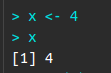
\includegraphics[scale=0.6]{r_assign_4.png}
\end{center}
We can see all of the names we have assigned in the \textit{environment} tab in the top right of RStudio
\begin{center}
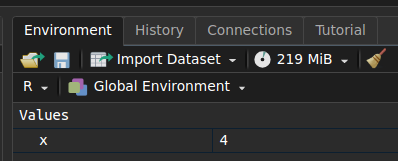
\includegraphics[scale=0.5]{r_env.png}
\end{center}
\end{frame}

\begin{frame}{How is data stored in R?}
Once names have been assigned, we can use just as we would their assigned values

\begin{center}
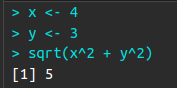
\includegraphics[scale=0.75]{sum_sq.png}
\end{center}

\end{frame}



\begin{frame}{Basic Elements of R}
\begin{enumerate}
\item Vectors
	\begin{itemize}
	\item All of one ``type"
	\item Can be short or long
	\end{itemize}
\item Data frames
	\begin{itemize}
	\item Shaped like a rectangular table
	\item Rows are observations, columns are variables (vectors)
	\end{itemize}
\item Functions
	\begin{itemize}
	\item Prewritten pieces of code
	\item Useful for performing common tasks
	\item Things like \texttt{mean()}, \texttt{sqrt()} or \texttt{plot()}
	\end{itemize}
\end{enumerate}
\end{frame}


\begin{frame}{Data in Practice}
We often uses a tabular form to store observations (rows) and variables (columns). This makes it simple to add or remove observations and variables with relative ease

\vspace{2mm}

\begin{table}[ht]
\centering
\begin{tabular}{rrllllr}
  \hline
Total Bill & Tip & Sex & Smoker & Day & Time & Size \\ 
  \hline
13.42 & 1.58 & Male & Yes & Fri & Lunch &   2 \\ 
  16.27 & 2.50 & Female & Yes & Fri & Lunch &   2 \\ 
  10.09 & 2.00 & Female & Yes & Fri & Lunch &   2 \\ 
  20.45 & 3.00 & Male & No & Sat & Dinner &   4 \\ 
  13.28 & 2.72 & Male & No & Sat & Dinner &   2 \\ 
  22.12 & 2.88 & Female & Yes & Sat & Dinner &   2 \\ 
  24.01 & 2.00 & Male & Yes & Sat & Dinner &   4 \\ 
  15.69 & 3.00 & Male & Yes & Sat & Dinner &   3 \\ 
%  11.61 & 3.39 & Male & No & Sat & Dinner &   2 \\ 
%  10.77 & 1.47 & Male & No & Sat & Dinner &   2 \\ 
%  15.53 & 3.00 & Male & Yes & Sat & Dinner &   2 \\ 
  \vdots & \vdots & \vdots & \vdots & \vdots & \vdots & \vdots \\
%  10.07 & 1.25 & Male & No & Sat & Dinner &   2 \\ 
%  12.60 & 1.00 & Male & Yes & Sat & Dinner &   2 \\ 
%  32.83 & 1.17 & Male & Yes & Sat & Dinner &   2 \\ 
%  35.83 & 4.67 & Female & No & Sat & Dinner &   3 \\ 
%  29.03 & 5.92 & Male & No & Sat & Dinner &   3 \\ 
%  27.18 & 2.00 & Female & Yes & Sat & Dinner &   2 \\ 
%  22.67 & 2.00 & Male & Yes & Sat & Dinner &   2 \\ 
%  17.82 & 1.75 & Male & No & Sat & Dinner &   2 \\ 
%  18.78 & 3.00 & Female & No & Thur & Dinner &   2 \\ 
   \hline
\end{tabular}
\end{table}

\end{frame}

\begin{frame}{Data in Practice}
In R, tabular data is typically stored as a \texttt{data.frame}
\begin{center}
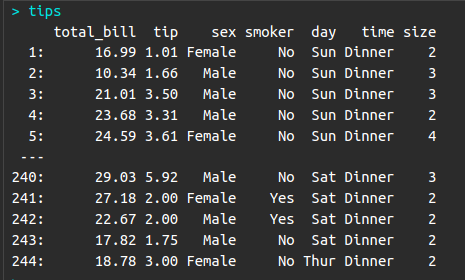
\includegraphics[scale=0.5]{r_tips.png}
\end{center}
\end{frame}

\begin{frame}{Using R Markdown}
R Markdown describes a specific type of file that is used in R (.Rmd) \vspace{3mm}

Uses \textit{markdown} language to easily add headers, or write things in \textbf{bold} or \textit{italics} \vspace{3mm}

Alongside written text allows us to write and compute R code \vspace{3mm}

Can be knit into pdf and submitted to gradescope

\begin{center}
%
\includegraphics[scale=0.12]{cat_yarn.jpg}

\includegraphics[scale=0.15]{cat_yarn2.png}
\end{center}

\end{frame}


\begin{frame}{Go forth and conquer}
\begin{enumerate}
\item Find lab on course website
\item Do it
\end{enumerate}
\end{frame}

%\begin{frame}
%\begin{columns}
%
%  \begin{column}{0.45\textwidth}
%%
%  \end{column}
%  \begin{column}{0.45\textwidth}
%%
%  \end{column}
%
%\end{columns}
%\end{frame}



%%%%%%%%%%%%%%%%


\end{document}
